\documentclass[prl,twocolumn]{revtex4-1}

\usepackage{graphicx}
\usepackage{color}
\usepackage{latexsym,amsmath}

\definecolor{linkcolor}{rgb}{0,0,0.65} %hyperlink
\usepackage[pdftex,colorlinks=true, pdfstartview=FitV, linkcolor= linkcolor, 
    citecolor= linkcolor, urlcolor= linkcolor, hyperindex=true,hyperfigures=true]{hyperref} %hyperlink%

% Ensure Arabic section numbering instead of Roman numerals
\renewcommand{\thesection}{\arabic{section}}
\renewcommand{\thesubsection}{\thesection.\arabic{subsection}}

\makeatletter
\renewcommand{\section}{\@startsection{section}{1}{\z@}%
    {-3.5ex \@plus -1ex \@minus -.2ex}{2.3ex \@plus.2ex}%
    {\normalfont\bfseries\raggedright}}

\renewcommand{\subsection}{\@startsection{subsection}{2}{\z@}%
    {3.5ex \@plus 1ex \@minus .2ex}{-1em}%
    {\normalfont\bfseries\raggedright}}
\makeatother

\begin{document}

\setcounter{secnumdepth}{1}

\title{Unsupervised Learning and Log-likelihood Analysis with Restricted Boltzmann Machines}

\author{Elias Maria Bonasera}
\author{Alberto Casellato}
\author{Nicola Garbin}
\author{Francesco Pazzocco}

\date{\today}

\begin{abstract}
\textit{We present a comprehensive study on the use of restricted Boltzmann machines (RBMs) for unsupervised learning of handwritten digit features from the MNIST dataset. Through experiments with a custom Python implementation, we focus on the RBM architecture, the training via Contrastive Divergence, and extensive hyperparameter tuning. We detail the experimental setup, the log-likelihood estimation method, and evaluate different configurations. The results highlight both the strengths and limitations of the approach, suggesting directions for future improvements.}
\end{abstract}

\maketitle

%%%%%%%%%%%%%%%%%%%%%%%%%%%%%%%%%%%%%%%%%%%%%%%%%%%%%%%%%%%%%%%%%%%%%%
% 1. Introduction
%%%%%%%%%%%%%%%%%%%%%%%%%%%%%%%%%%%%%%%%%%%%%%%%%%%%%%%%%%%%%%%%%%%%%%
\section*{Introduction}
\textit{Unsupervised learning is essential for extracting features from unlabeled data, and probabilistic graphical models (PGMs), such as Markov Random Fields (MRFs), provide a framework for this task. Restricted Boltzmann Machines (RBMs) are a specific type of MRF with a bipartite structure (a visible and a hidden layer with no intra-layer connections). Their ability to model complex distributions and learn efficient representations of intricate data relatively fast makes them interesting both theoretically and for practical applications \cite{intro_ML,bortoletto, practical}.}

In this work, we present a complete implementation of a Restricted Boltzmann Machine (RBM) and analyze its behavior through systematic experiments. The paper is organized as follows:
Section~\ref{sec:theory} presents the theoretical foundation of RBMs, Section~\ref{sec:methodology} details the experimental methodology and implementation specifics, Section~\ref{sec:results} shows the experimental results accompanied by graphical analysis, and Section~\ref{sec:discussion} discusses our findings, draws conclusions, and suggests avenues for future research. Supplementary equations and technical details are provided in the Appendix.

%%%%%%%%%%%%%%%%%%%%%%%%%%%%%%%%%%%%%%%%%%%%%%%%%%%%%%%%%%%%%%%%%%%%%%
% 2. Theory: Restricted Boltzmann Machines
%%%%%%%%%%%%%%%%%%%%%%%%%%%%%%%%%%%%%%%%%%%%%%%%%%%%%%%%%%%%%%%%%%%%%%
\section{Theory}
\label{sec:theory}
\subsection{Restricted Boltzmann Machines}
RBMs are generative models consisting of a visible layer, representing the input data, and a hidden layer that captures latent features.

Mathematically, RMBs consist in a set of $D$ binary visible units $i$ of state $\{v_i\}_{i=1, ..., D}$ symmetrically connected to a set of $L$ binary hidden units $\mu$ of state $\{h_\mu\}_{\mu=1, ..., L}$. The continuos weight $w_{i\mu}$ quantifies the strength between unit $i$ and unit $\mu$ (see Figure~\ref{fig:RBM_architecture}). \cite{intro_ML,bortoletto}. 

The energy of a configuration $(\mathbf{v},\mathbf{h})$ is defined as
\begin{equation}
	E(\mathbf{v},\mathbf{h}) = -\sum_{i} a_i v_i - \sum_{\mu} b_\mu h_\mu - \sum_{i,\mu} v_i w_{i\mu} h_\mu,
\end{equation}
where $a_i$ and $b_\mu$ are the biases for the visible and hidden units, respectively, and $w_{i\mu}$ denotes the weight between them. No intra-layer connections exist, which simplifies the energy function and learning dynamics. 

\begin{figure}[!tb]
	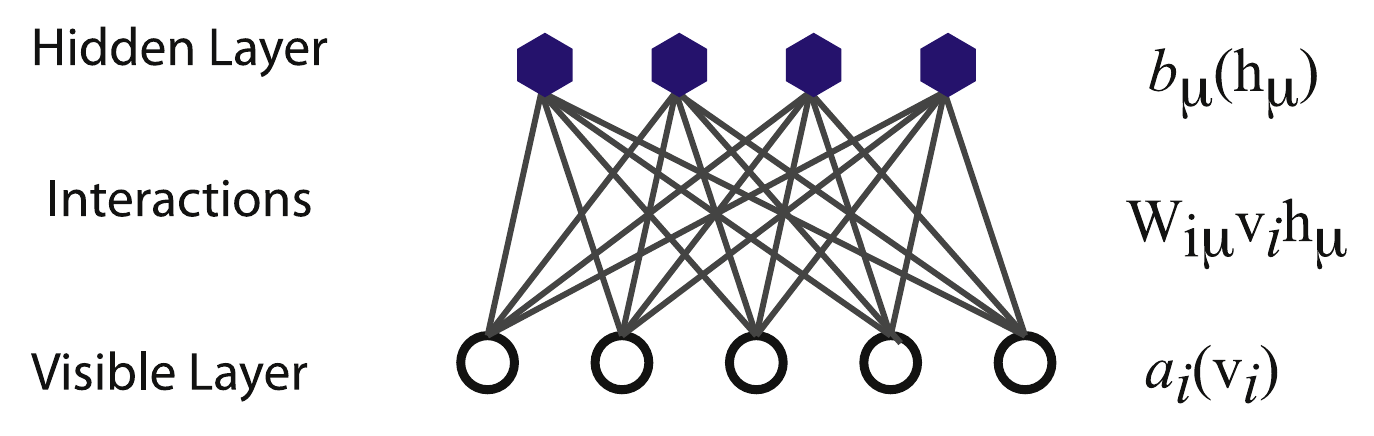
\includegraphics[width=0.44\textwidth]{RBM_structure.png}
	\caption{Bipartite structure of a Restricted Boltzmann Machine. Visible units (bottom) are connected to hidden units (top) with no intra-layer connections.}
	\label{fig:rbm_model}
\end{figure}

The probability of a hidden unit being active is computed using the logistic sigmoid for both visibile and hidden units:
\begin{equation}
	p(h_\mu=1|\mathbf{v}) = \sigma\left(b_\mu+\sum_{i}v_iw_{i\mu}\right),
	\label{eq:p_of_h}
\end{equation}
\begin{equation}
	p(v_i=1|\mathbf{h}) = \sigma\left(a_i+\sum_{\mu}h_\mu w_{i\mu}\right).
	\label{eq:p_of_v}
\end{equation}
The training consists in the minimization of the energy's $\boldsymbol{\theta}$ parameters; and is typically performed via Contrastive Divergence algorithm, which approximates the gradient of the log-likelihood by alternating Gibbs sampling between the visible and hidden layers \cite{bortoletto,practical,intro_ML}.

%%%%%%%%%%%%%%%%%%%%%%%%%%%%%%%%%%%%%%%%%%%%%%%%%%%%%%%%%%%%%%%%%%%%%%
% 3. Methodology
%%%%%%%%%%%%%%%%%%%%%%%%%%%%%%%%%%%%%%%%%%%%%%%%%%%%%%%%%%%%%%%%%%%%%%
\section{Methodology}
\label{sec:methodology}
\subsection{Experimental Setup and Preprocessing}
The MNIST dataset is used, consisting of 60,000 training images and 10,000 handwritten digit test images. Each image is flattened into a 784-dimensional vector and binarized by thresholding at 0.5. Two encoding schemes are implemented:
\begin{itemize}
	\item \textbf{Bernoulli encoding:} Pixel values in $\{0,1\}$.
	\item \textbf{Spin encoding:} Pixel values in $\{-1,+1\}$.
\end{itemize}
The RBM is implemented in a Python class (\texttt{RBM}) with configurable hyperparameters such as the number of hidden units, learning rate, optimizer type (SGD or RMSprop), regularization strength, and choice of encoding.

\subsection{Log-Likelihood Estimation and Parameter Tuning}
Performance is evaluated using the log-likelihood metric, computed as:
\begin{equation}
	\mathcal{L} = \frac{1}{M}\sum_{m=1}^{M} \log \left(\sum_{\mathbf{h}} e^{-E(\mathbf{v}^{(m)},\mathbf{h})}\right) - \log Z,
	\label{eq:loglikelihood}
\end{equation}
where $Z$ is the partition function. 
Due to the computational difficulty of calculating $Z$, we employ approximations; for the mathematical analysis, see~\ref{sec:app}

Hyperparameters varied in our experiments include:
\begin{itemize}
	\item Number of hidden units (e.g., 3 to 13).
	\item Number of Contrastive Divergence steps ($k=1,2,3$).
	\item Learning rate and regularization coefficients.
	\item Optimizer type (SGD versus RMSprop).
	\item Data encoding: Bernoulli vs. Spin.
\end{itemize}
For each configuration, training is repeated over multiple runs (with different random seeds) to ensure statistical significance.

%%%%%%%%%%%%%%%%%%%%%%%%%%%%%%%%%%%%%%%%%%%%%%%%%%%%%%%%%%%%%%%%%%%%%%
% 4. Results
%%%%%%%%%%%%%%%%%%%%%%%%%%%%%%%%%%%%%%%%%%%%%%%%%%%%%%%%%%%%%%%%%%%%%%
\section{Results}
\label{sec:results}
Experimental results are presented using several figures. For instance, Figure~\ref{fig:L_of_epochs} illustrates the evolution of the log-likelihood over training epochs, showing convergence after approximately 150 epochs. Figure~\ref{fig:L_of_CD} compares the effects of different Contrastive Divergence steps. Additional graphs (e.g., Figure~\ref{fig:L_of_L}) display the impact of varying the number of hidden units. In general, we observe:
\begin{itemize}
	\item Steady improvement of log-likelihood with training, saturating after a sufficient number of epochs.
	\item Marginal gains when increasing the number of CD steps, with CD-1 already offering a reasonable trade-off.
	\item Increased hidden units enhance performance up to a point, beyond which improvements plateau.
	\item One-hot hidden activations (POTS) and spin encoding can lead to instability or degraded performance.
\end{itemize}

\begin{figure}[!tb]
	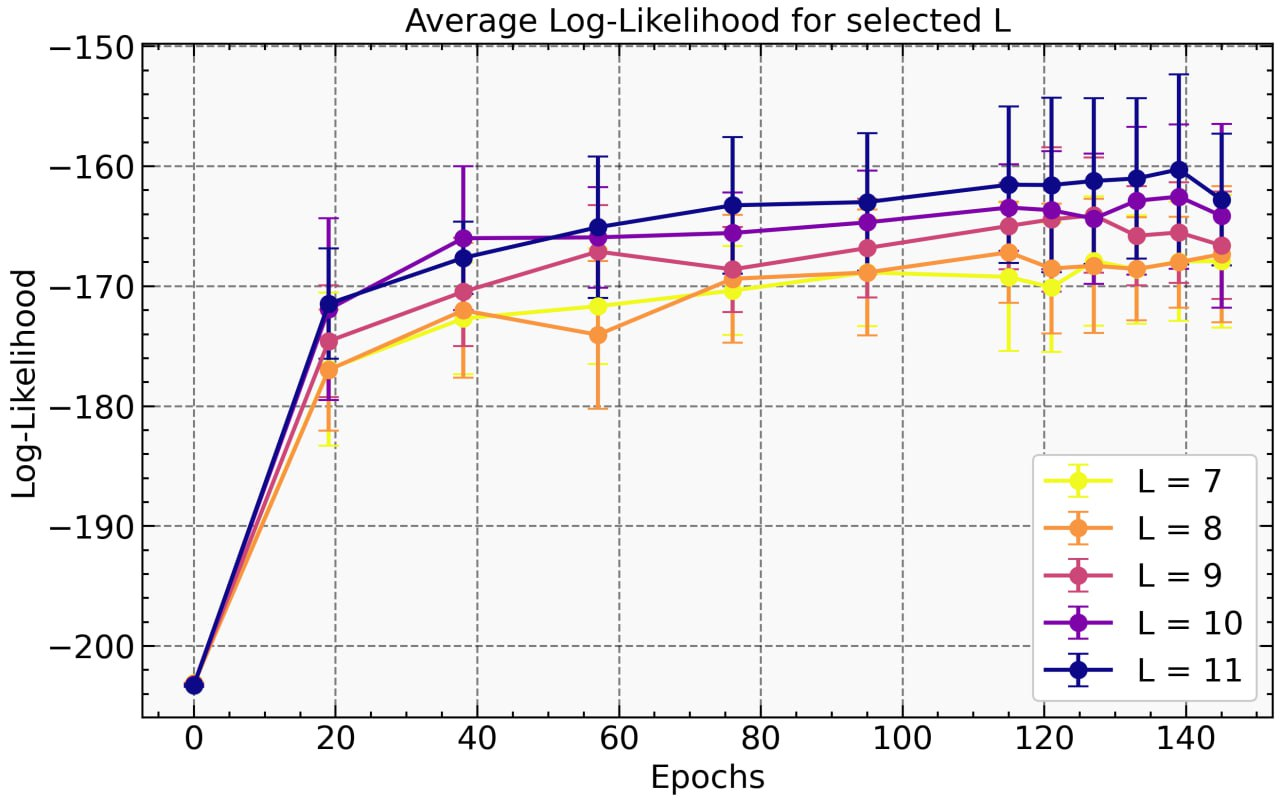
\includegraphics[width=0.44\textwidth]{L_of_epochs.jpg}
	\caption{Evolution of the log-likelihood over training epochs. Results are averaged over multiple runs.}
	\label{fig:L_of_epochs}
\end{figure}

\begin{figure}[!tb]
	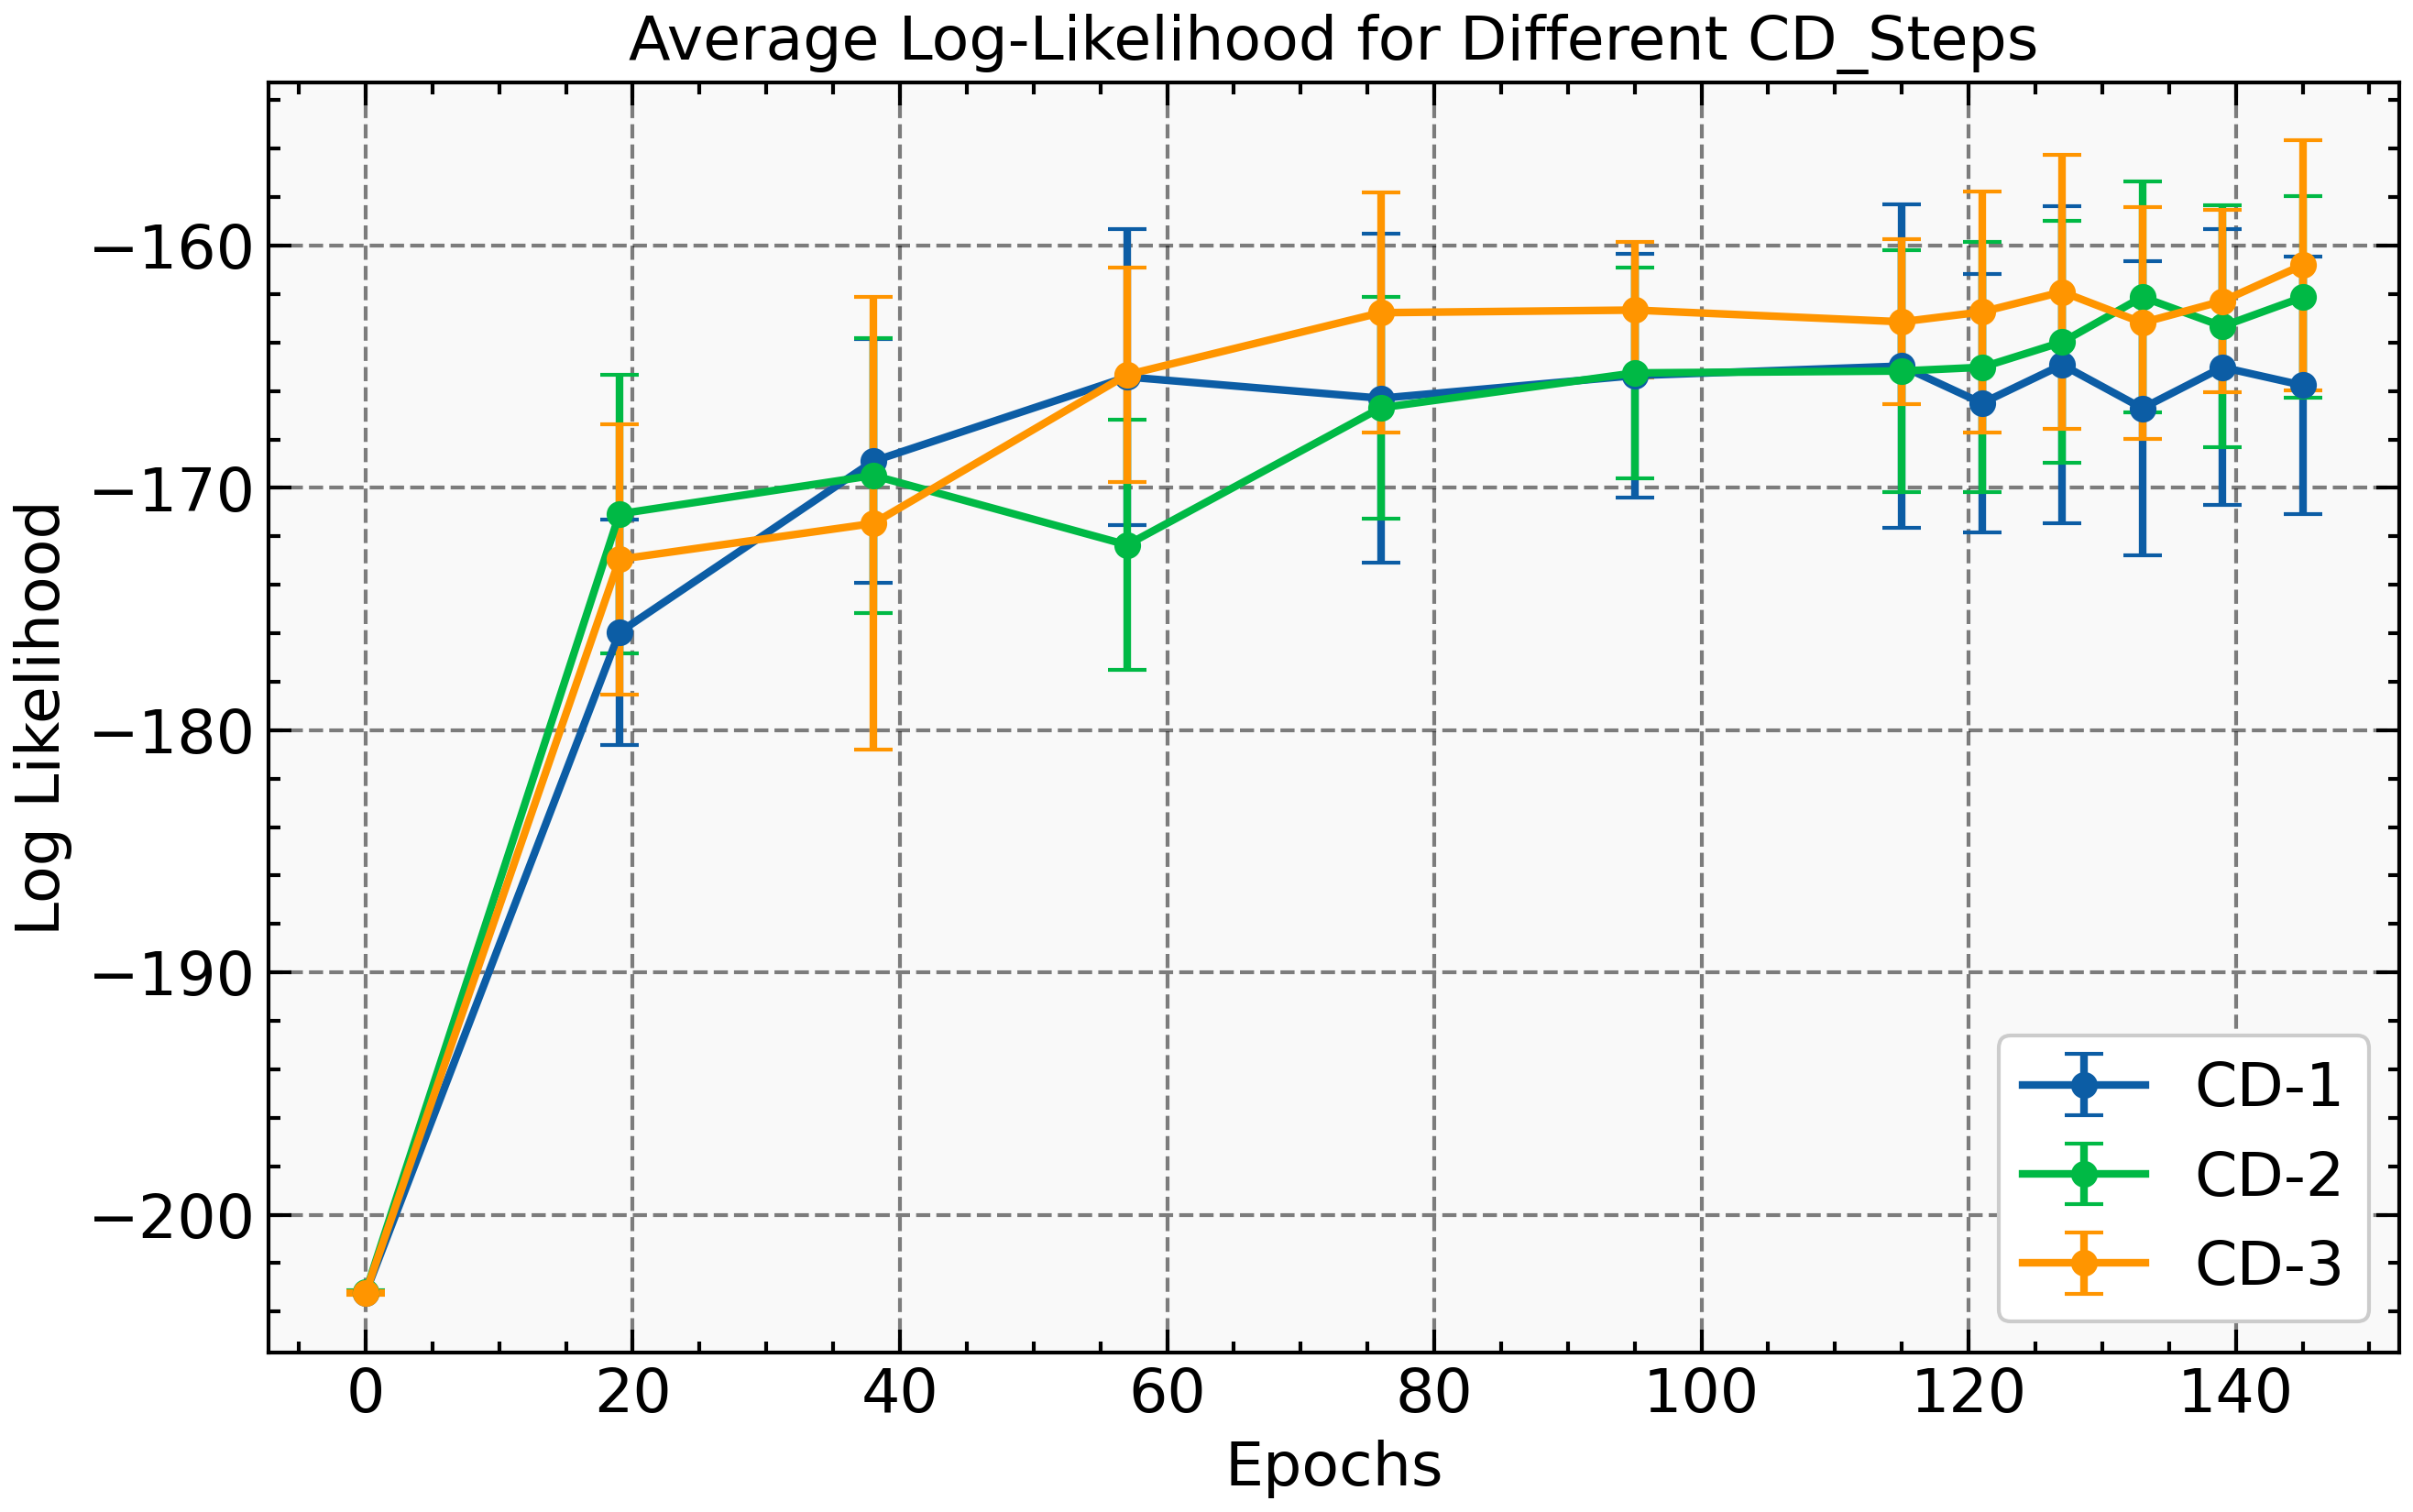
\includegraphics[width=0.44\textwidth]{L_of_CD.png}
	\caption{Log-likelihood evolution for different numbers of Contrastive Divergence steps.}
	\label{fig:L_of_CD}
\end{figure}

%%%%%%%%%%%%%%%%%%%
\begin{figure}[!tb]
	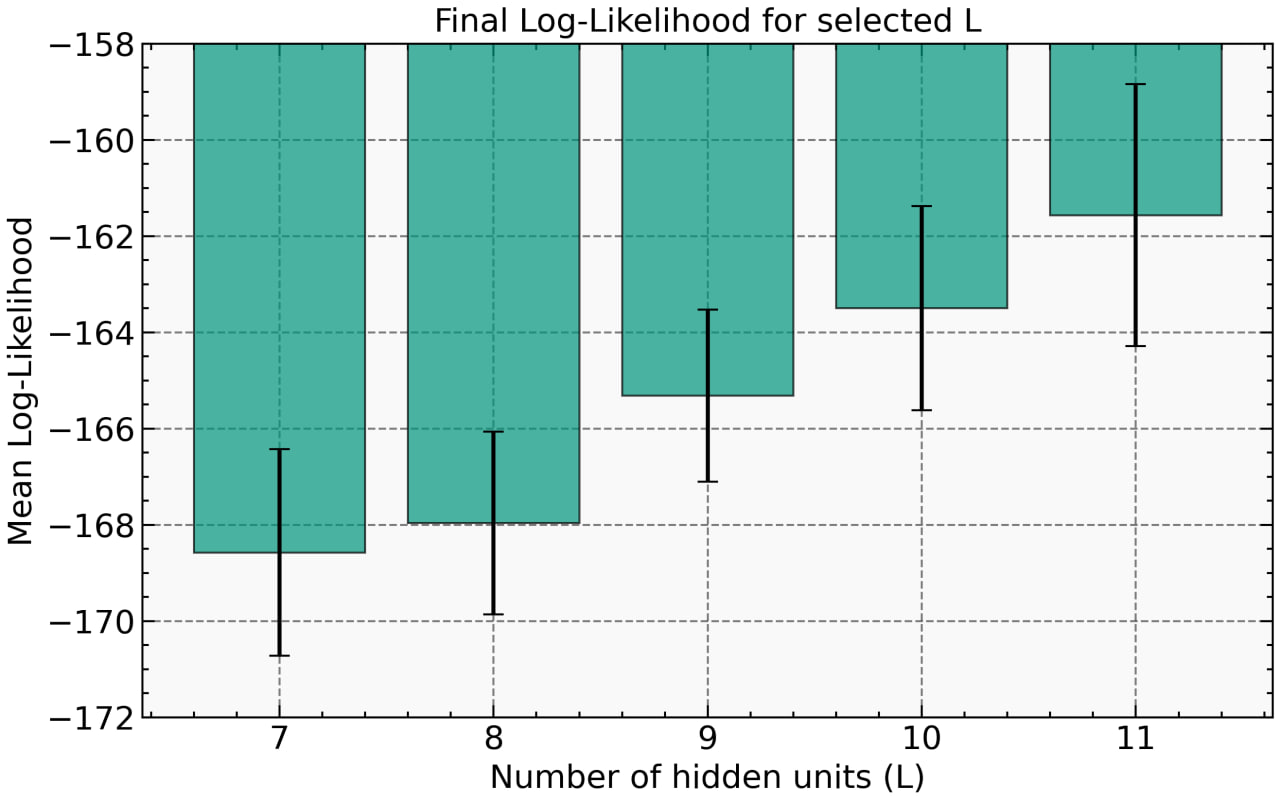
\includegraphics[width=0.44\textwidth]{L_of_L.jpg}
	\caption{Bar chart displaying the weighted mean and standard deviation of the log-likelihood over the last epochs for different values of L.}
	\label{fig:L_of_L}
\end{figure}
%%%%%%%%%%%%%%%%%%%

%%%%%%%%%%%%%%%%%%%
\begin{figure}[!tb]
	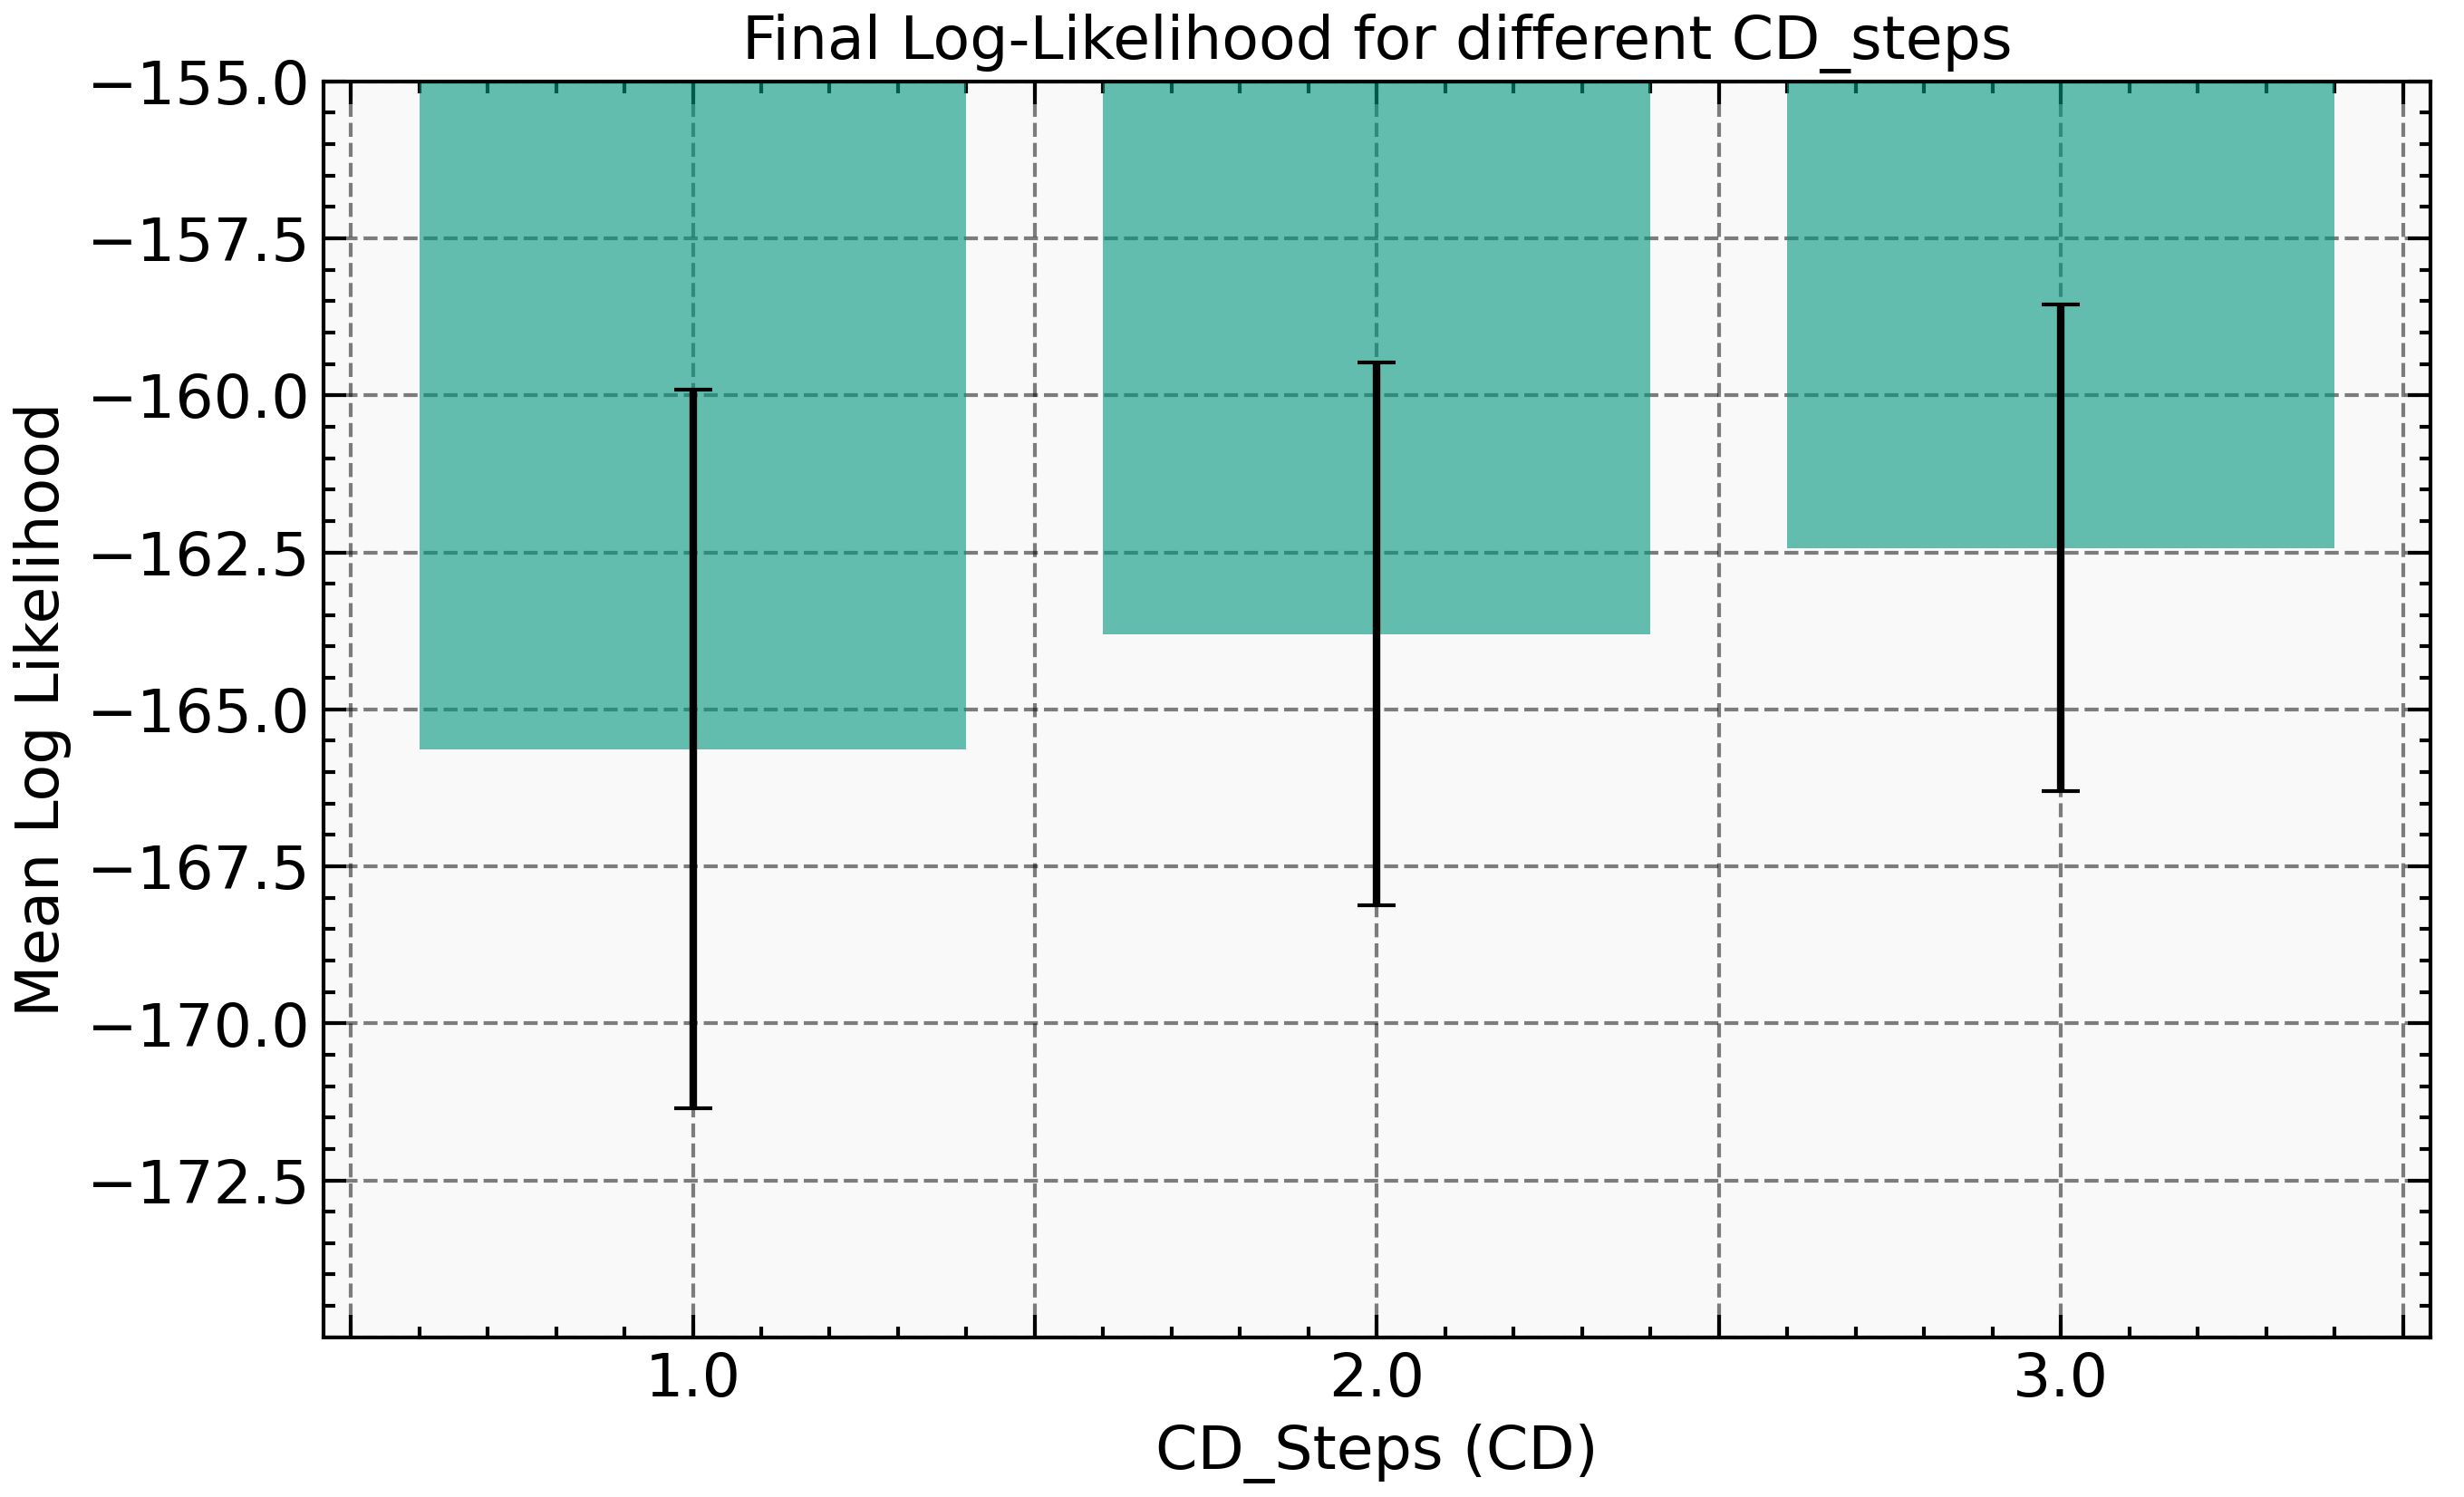
\includegraphics[width=0.455\textwidth]{final_L_of_CD.png}
	\caption{Bar chart displaying the weighted mean and standard deviation of the log-likelihood over the last epochs for different numbers of CD steps.}
	\label{fig:final_L_of_CD}
\end{figure}
%%%%%%%%%%%%%%%%%%%

%%%%%%%%%%%%%%%%%%%%%%%%%%%%%%%%%%%%%%%%%%%%%%%%%%%%%%%%%%%%%%%%%%%%%%
% 5. Discussion and Conclusion
%%%%%%%%%%%%%%%%%%%%%%%%%%%%%%%%%%%%%%%%%%%%%%%%%%%%%%%%%%%%%%%%%%%%%%
\section{Discussion and Conclusion}
\label{sec:discussion}
Our experiments confirm that RBMs are capable of learning useful representations of handwritten digits in an unsupervised fashion. The analysis shows that:
\begin{itemize}
	\item Proper initialization and regularization are critical for stable training.
	\item While increasing hidden units improves performance, the benefit saturates beyond a certain network capacity.
	\item The choice of optimizer and data encoding significantly affects convergence dynamics.
\end{itemize}
These findings provide a baseline for further research, which might include adaptive scheduling of CD steps, deeper architectures (e.g., stacked RBMs), or alternative estimation techniques (such as AIS). Overall, the work not only demonstrates the practical viability of RBMs but also highlights their limitations and areas for future improvement.

%%%%%%%%%%%%%%%%%%%%%%%%%%%%%%%%%%%%%%%%%%%%%%%%%%%%%%%%%%%%%%%%%%%%%%
% 6. Appendix
%%%%%%%%%%%%%%%%%%%%%%%%%%%%%%%%%%%%%%%%%%%%%%%%%%%%%%%%%%%%%%%%%%%%%%
\section{Appendix}
\subsection*{Gradient Update Equations and Regularization}
\begin{equation}
	\boldsymbol{\theta}_{t+1}=\boldsymbol{\theta}_t-\gamma\cdot\eta_t\cdot\text{sign}(\boldsymbol{\theta}),
	\label{eq:regu}
\end{equation}
\begin{equation}
	\boldsymbol{\theta}_{t+1}=\boldsymbol{\theta}_t\pm\eta_t\nabla_{\boldsymbol{\theta}}E(\boldsymbol{\theta}),
	\label{eq:sgd}
\end{equation}
\begin{equation}
	\begin{cases}
		\boldsymbol{g}_t=\nabla_{\boldsymbol{\theta}}E(\boldsymbol{\theta}), \\
		\boldsymbol{s}_t=\beta\boldsymbol{s}_{t-1}+(1-\beta)\boldsymbol{g}_t^2, \\
		\boldsymbol{\theta}_{t+1}=\boldsymbol{\theta}_t\pm\eta_t\frac{\boldsymbol{g}_t}{\sqrt{\boldsymbol{s}_t+\epsilon}}.
	\end{cases}
	\label{eq:rmsprop}
\end{equation}

\subsection*{Log-likelihood and Partition Function Approximations}
$\mathcal{L}$ of the data:

\begin{equation}
	\mathcal{L}=\frac{1}{M}\sum_{m=1}^{M}{\ell_{\theta}(v^{(m)})}
	\label{eq:Loglikelihood}
\end{equation}
\begin{equation}
	\ell_{\theta}(v^{(m)})=\log\sum_{h}{e^{-E(v,h)}-\log{Z}}
	\label{eq:loglikelihood}
\end{equation}

where $M$ is the number of data points, $Z$ is the partition function, $E(v,h)$ in the exponential argument $e^{-E(v,h)}=G(h)\prod_{i}{e^{H_i(h)v_i}}$ is the energy function, with $G(h)=\prod_{\mu}{e^{b_{\mu}h_{\mu}}}$ and $H_i(h)=a_i+\sum_{\mu}w_{i\mu}h_\mu$, and, in Eq.~\ref{eq:loglikelihood}, the index $h$ of the summation represents each possible state of the hidden layer.


$Z$ approximations (including second-order Taylor expansion) and normalization techniques (e.g., using a scaling factor in the Bernoulli case or approximating $2\cosh(H_i)$ for spin encoding) are greatly discussed in \cite{baiesi} here we report the final $Z$.
For Bernoulli units, the partition function is manipulated as:
\begin{equation}
	Z = q^D\sum_{\mathbf{h}} G(\mathbf{h}) \prod_{i=1}^D \frac{1+e^{H_i(\mathbf{h})}}{q},
	\label{eq:Z_function_bernulli}
\end{equation}

and for spin encoding:
\begin{equation}
	Z = \sum_{\mathbf{h}} G(\mathbf{h}) \prod_{i=1}^D 2\cosh\left(H_i(\mathbf{h})\right).
	\label{eq:Z_function_spin}
\end{equation}

% Bibliography
\bibliography{biblio}
\bibliographystyle{apsrev4-1}

\end{document}